\documentclass[a4paper,12pt]{article}

\usepackage{ProfModels}



 
\begin{document}

\begin{Maquette}[DM]{Niveau=1, Numero=4, Date=19/10/2024,Semestre=2, FinDate=20/12/2024}

\begin{exercice}
\begin{enumerate}
\item Compléter les expressions par qui convient :
\begin{tasks}[style=itemize](2)
\task $8x = 2x + \cdots$
\task $14xy = 2x \times \cdots$
\task $146ab = 200ab - \cdots$
\task $52 x = 12 x + \cdots$

\end{tasks}
\item Réduire ce qui suit :
\begin{tasks}[style=itemize](3)
\task $3x+2+6x-7$
\task $5ab-1+3ab-8-14ab$
\task $6a^{2}+a-3a^{2}-5a+4$
\end{tasks}
\item Développer et réduire les produits suivants:
\begin{tasks}[style=itemize](2)
\task $-7x(2x+1)$
\task $5ab(2ab+3a-8b)$
\task $(2x+4)(5x+8)$
\task $(6x-7)(5x-2)$
\end{tasks}
\item Factoriser :
\begin{tasks}[style=itemize](4)
\task $8x-8y$
\task $25ab+5$
\task $49x^{2}+56y^{3}$
\end{tasks}
\end{enumerate}
\end{exercice}

\begin{exercice}
Résoudre les équations suivantes :
\begin{tasks}[style=itemize](3)
\task $x+4=2$
\task $7+a=-3$
\task $-4-x=1$
\task $2+x=-x+1$
\task $3x-5=6$
\task $4(3x-1)=2x-3$
\task $-2x+6=-4x-8$
\task $12b-1=5b-17$
\task $-7a-9=-15-a$
\end{tasks}
\end{exercice}

\begin{exercice}
\begin{tikzpicture}
\tkzDefPoints{0/0/A,5/0/B,5/3/C,0/3/D}
\tkzDrawSegments(A,B B,C C,D D,A)

\tkzLabelPoint[left](A){A}
\tkzLabelPoint[below right=5pt](B){B}
\tkzLabelPoints[above](C,D)
\tkzDrawSegment[dim={$x$,-0.5cm,below=5pt}](A,B)
\tkzDrawSegment[dim={$y$,0.3cm,right=5pt}](C,B)

\end{tikzpicture}
\end{exercice}
\end{Maquette}
\end{document}
